\documentclass[12pt]{nmsuth01}
%If your system does not have a latex package ``pkg'', for example,
 %attempting to run latex on the file will produce an error report
 %reading something like ``Latex error:  File pkg.sty not found.''
%
%Your system should have the latex symbol package.  If not comment out 
 %the next line by placing a percent sign % at the beginning of the line.
\usepackage{latexsym}
%Your system may not have the American Mathematical Society packages
 %for mathematics and theorem formatting.  If not, comment out the
 %next line.  If you comment out the next line, you should also
 %comment out all the theorem formatting commands, and you should not
 %try to process the part of the document called chp1a.tex.  Commment
 %out the line below calling for \input{chp1a}.
\usepackage{amsmath,amsthm}
%Your system may not have the xypic drawing package.  If not, comment
 %out the next line.  If you comment out the next line, you should
 %also not try to process chp1a.tex.  
\usepackage[all]{xy}
%Your system should have the graphicx package for included graphics.
 %If not, or, if you have no graphics to include, comment out the next 
 %line.  If you commment out the next line, then you should not try to 
 %process the part of the document called graphics.tex.  Comment out
 %the line below calling for \section{SAMPLE TEXT WITH GRAPHICS} \label{graphics}
%This file illustrates how include in your thesis graphical
 %output.
%The next line produces an indented paragraph to start the document
 %unit.  The LaTeX defaults start most units without indentations.
\hspace{\parindent}
This is sample text with graphics.
\begin{figure}[h]
  \centering
  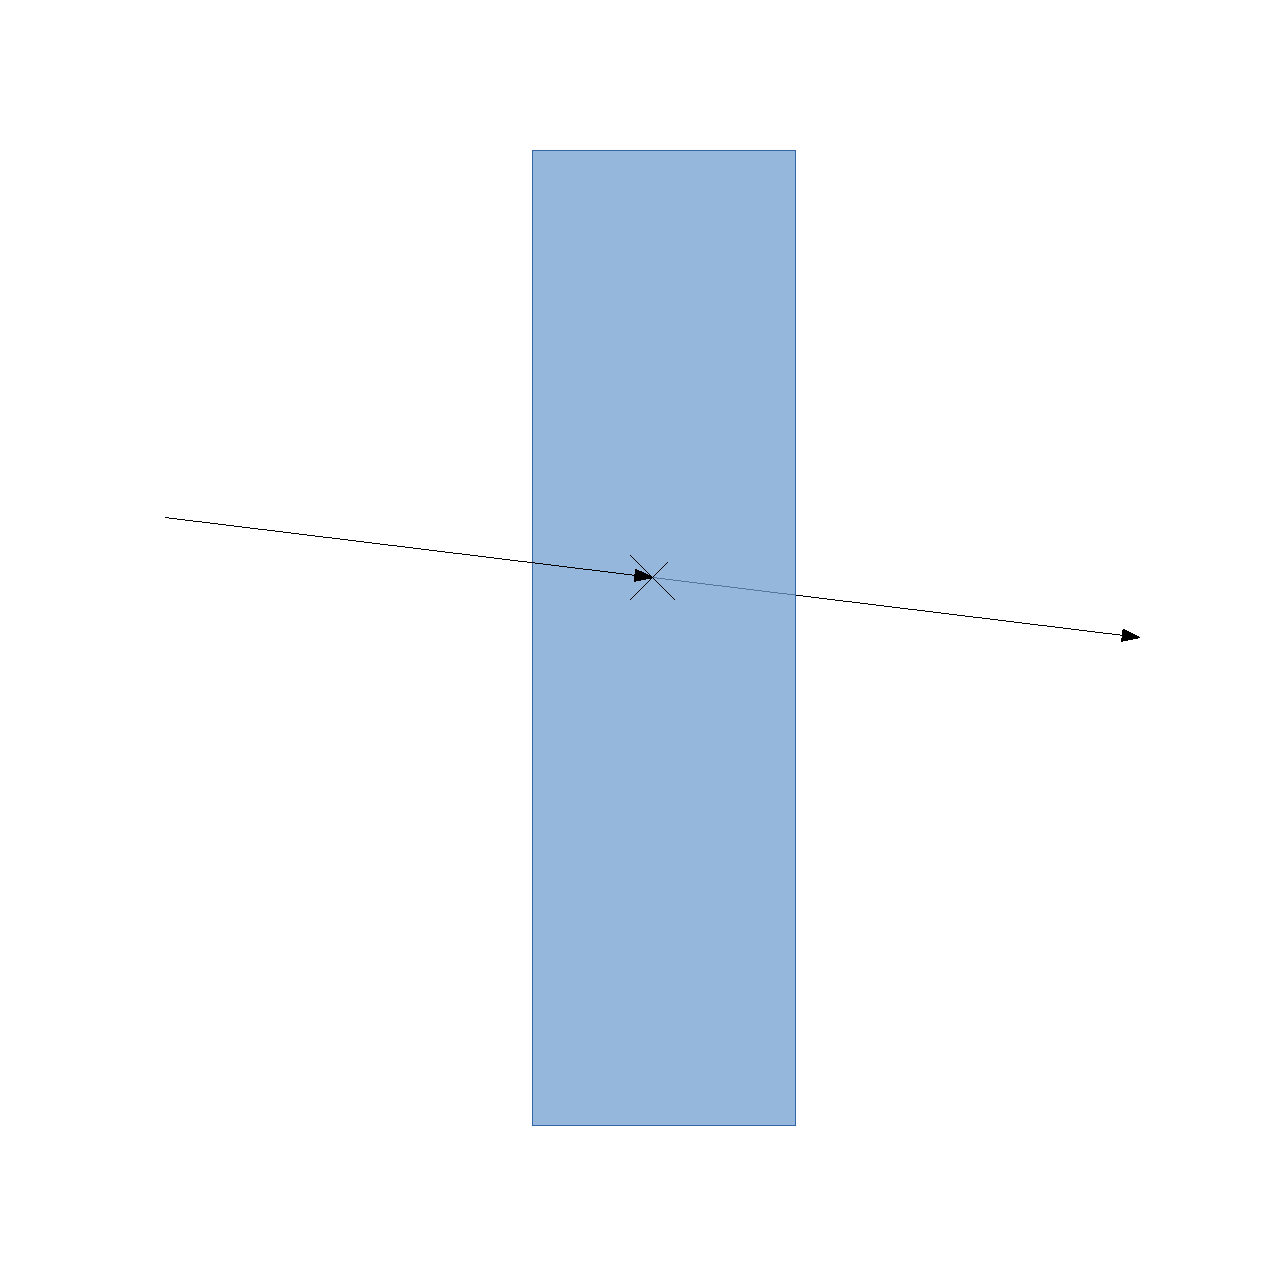
\includegraphics[angle=-90,width=4in]{figures/bz.pdf}
  \caption{This is an inserted EPS graphic}
  \label{fig:mygraph1}
\end{figure}
Sample ref of \ref{fig:mygraph1} 

\begin{figure}[t]
 \centering
  \includegraphics[angle=-90, width=4in]{figures/E734eta.pdf}  
    \caption{This is another inserted PDF graphic}
    \label{fig:mygraph2}
\end{figure}
%This is the end of the file graphics.tex


\usepackage{graphicx}
\usepackage{subcaption}
%The next settings give the correct margins for an NMSU Ph.D. thesis.
\setlength{\evensidemargin}{0.5in}
\setlength{\oddsidemargin}{0.5in}
\setlength{\textwidth}{5.75in}
\setlength{\topmargin}{-0.25in}
\setlength{\textheight}{8.25in}
%
%
% Theorem Formatting Commands.
\theoremstyle{plain}
\newtheorem{lemma}{Lemma}[section]
\newtheorem{prop}{Proposition}[section]
\newtheorem{theorem}{Theorem}[section]
\newtheorem{cor}{Corollary}[section]
%\newtheorem*{nametheorem}{Theorem}[section]
\theoremstyle{definition}
\newtheorem{defn}{Definition}[section]
\newtheorem{example}{Example}[section]
\theoremstyle{remark}
\newtheorem*{rem}{Remark}
\newtheorem*{convention*}{Convention}
%
% Miscellaneous Special Capitals
\newcommand{\bZ}{{\mathbf Z}}
\newcommand{\bQ}{{\mathbf Q}}
\newcommand{\bR}{{\mathbf R}}
\newcommand{\cC}{{\mathcal C}}
% 
%Miscellaneous symbols
\newcommand{\op}{{\rm \oplus}}
\newcommand{\id}{\rm id}
%
%Miscellaneous Greek letters
\newcommand{\eps}{\ensuremath{\epsilon}}
\newcommand{\ga}{\ensuremath{\gamma}}
%
%Miscellaneous operators
\DeclareMathOperator{\Coker}{Coker}
\DeclareMathOperator{\Tor}{Tor}
\DeclareMathOperator{\Ext}{Ext}
\DeclareMathOperator{\Maps}{Maps}
\DeclareMathOperator{\Hom}{Hom}
\DeclareMathOperator{\Aut}{Aut}
\DeclareMathOperator{\Sin}{Sin}
\DeclareMathOperator{\Tot}{Tot}
\DeclareMathOperator{\im}{im}
%
%Prepare for  double spacing
%\renewcommand{\baselinestretch}{1.5}
\newlength{\singlespace}
\setlength{\singlespace}{\baselineskip}
\newlength{\doublespace}
\setlength{\doublespace}{2.0\baselineskip}
%
\begin{document}
%Use the next line to obtain double spacing for the main body of the document
\setlength{\baselineskip}{\doublespace}
%Comment out the preceding line and uncomment the next line containing
 %a \setlength command to obtain single spacing for the main body of 
 %the document.
%\setlength{\baselineskip}{\singlespace}
%
%Why do you care about this option?
%There are two answers.  One is that it takes less paper to print a
 %preliminary draft of the thesis.  The second is that singlespacing
 %makes the structural units of the document more apparent.  Single
 %spacing makes it easy to identify definitions, lemmas, theorems, and 
 %so on, and it makes apparent such problems as a paragraph that is
 %running too long. On the other hand, the double spacing is good for 
 %checking for typographical errors in a manuscript.  Note that a 
 %document printed in singlespacing and doublespacing formats will 
 %have its problems with page and line breaks in different locations.  
%
%The title page, approval page, dedication page, acknowledgment page,
 %vita page, abstract page, and pages listing tables and figures (if
 %there are any) all carry roman numerals.
\pagenumbering{roman}
\pagestyle{empty}
%This file makes a title page for a Ph.D. thesis.
\thispagestyle{empty}
\renewcommand{\baselinestretch}{2}
\begin{center}
NEUTRAL CURRENT ELASTIC SCATTERING \\ AND THE STRANGE SPIN STRUCTURE OF THE PROTON
\vspace{0.1in}
BY\\
\vspace{0.1in}
KATHERINE WOODRUFF
\end{center}
\vspace{1.0in}
\begin{center}
A dissertation submitted to the Graduate School\\
\vspace{0.1in}
in partial fulfillment of the requirements\\
\vspace{0.1in}
for the degree \\
\vspace{0.1in}
Doctor of Philosophy
\end{center}
\vfill
\begin{center}
Major Subject: Physics
\end{center}
\vspace{1.0in}
\begin{center}
New Mexico State University\\
\vspace{0.1in}
Las Cruces New Mexico\\
\vspace{0.1in}
November 2018
\end{center}
\newpage
%This is the end of the title page.

\pagestyle{plain}
%This file makes the approval page for a Ph.D. thesis at NMSU.  It
 %must be replaced when a permanent Dean of the Graduate School is named.
\noindent
``Neutral Current Elastic Scattering and the Strange Spin Structure of the Proton,'' 
a dissertation prepared by
Katherine Woodruff 
in partial fulfillment of the requirements for the degree, 
Doctor of Philosophy,
has been approved and accepted by the following:

\setlength{\baselineskip}{\singlespace}
\vspace{0.1in}
\begin{flushleft}
\hrulefill
\newline
Dr. Luis Cifuentes
\newline
Dean of the Graduate School
\vspace{0.5in}

\hrulefill
\newline
Vassili Papavassiliou
\newline
Chair of the Examining Committee
\vspace{0.5in}

\hrulefill
\newline
Date
\vspace{0.5in}
\newline
Committee in charge:
\end{flushleft}

\setlength{\baselineskip}{\doublespace}
Dr. Vassili Papavassiliou, Chair

Dr. Stephen Pate

Dr. Igor Vasiliev

Dr. Steven Stochaj

\newpage
%This is the end of the approval page.

%
%This file makes a dedication page.
\begin{center}
DEDICATION
\end{center}
%The next blank line is needed to have the dedication text
 %appropriately indented.

I dedicate this work to my mom, dad, sister, bill.

\newpage
%This is the end of the dedication page.

%
%This file makes a page for acknowledgments.
\begin{center}
ACKNOWLEDGMENTS
\end{center}
%The next blank line is needed to have the dedication text
 %appropriately indented.

I would like to thank my advisor, ...

\newpage
%This is the end of the page for acknowledgments.

%
%This file makes a vita page in the required two column format.
\begin{center}
            VITA
\end{center}
\begin{flushleft}
\begin{tabular}{ll}
2006-2009        &  A.S., Linn-Benton Community College, Albany, Oregon
\\
& \\
2009-2012        &  B.S., University of Oregon, Eugene, Oregon
\\
& \\
2012-2015        &  M.S., New Mexico State University, Las Cruces, New Mexico
\end{tabular}
\end{flushleft}
\vspace{0.1in}
\begin{center}PUBLICATIONS
\end{center}
  C. Adams \textit{at al.}, "A Deep Neural Network for Pixel-Level Electromagnetic Particle Identification in the MicroBooNE Liquid Argon Time Projection Chamber”," \textit{Submitted to: Phys. Rev. D}, 2018. \\
  C. Adams \textit{at al.}, "Comparison of Muon-Neutrino-Argon Multiplicity Distributions Observed by MicroBooNE to GENIE Model Predictions," \textit{Submitted to: Phys. Rev. D}, 2018. \\
  C. Adams \textit{at al.}, "Ionization Electron Signal Processing in Single Phase LAr TPCs II: Data/Simulation Comparison and Performance in MicroBooNE," \textit{JINST}, vol. 13, no. 07, p. P07007, 2018. \\
  C. Adams \textit{at al.}, "Ionization Electron Signal Processing in Single Phase LAr TPCs I: Algorithm Description and Quantitative Evaluation with MicroBooNE Simulation," \textit{JINST}, vol. 13, no. 07, p. P07006, 2018. \\
  R. Acciarri \textit{at al.}, "The Pandora Multi-Algorithm Approach to Automated Pattern Recognition of Cosmic Ray Muon and Neutrino Events in the MicroBooNE Detector," \textit{Eur. Phys. J.}, vol. C78, p. 82, 2018. \\
  R. Acciarri \textit{at al.}, "Measurement of Cosmic Ray Reconstruction Efficiencies in the MicroBooNE LAr TPC Using a Small External Cosmic Ray Counter," \textit{JINST}, vol. 12, no. 12, p. P12030, 2017. \\
  R. Acciarri \textit{at al.}, "Noise Characterization and Filtering in the MicroBooNE Liquid Argon TPC," \textit{JINST}, vol. 12, no. 08, p. P08003, 2017. \\
  R. Acciarri \textit{at al.}, "Michel Electron Reconstruction Using Cosmic-Ray Data from the MicroBooNE LArTPC," \textit{JINST}, vol. 12, no. 09, p. P09014, 2017. \\
  P. Abratenko \textit{at al.}, "Determination of Muon Momentum in the MicroBooNE LArTPC Using an Improved Model of Multiple Coulomb Scattering," \textit{JINST}, vol. 12, no. 10, p. P10010, 2017. \\
  R. Acciarri \textit{at al.}, "Convolutional Neural Networks Applied to Neutrino Events in a Liquid Argon Time Projection Chamber," \textit{JINST}, vol. 12, no. 03, p. P03011, 2017. \\
   R. Acciarri \textit{et al.}, "Design and Construction of the MicroBooNE Detector," \textit{JINST}, vol. 12, no. 02, p. P02017, 2017. \\
\begin{center}
FIELD OF STUDY
\end{center}
\begin{flushleft}
Major Field: Experimental Particle Physics
\end{flushleft}

\newpage
%This is the end of the vita page.

%
%This file makes an abstract for a Ph.D. thesis.
\begin{center}
ABSTRACT
\end{center}
\vspace{0.3in}
\begin{center}
THESIS\\ TITLE
\\
BY
\\
KATHERINE WOODRUFF
\end{center}
\vspace{0.3in}
\begin{center}
Doctor of Philosophy

New Mexico State University

Las Cruces, New Mexico, 201?

Dr. Vassili Papavassiliou, Chair
\end{center}
\vspace{0.3in}
%The next line produces an indented paragraph to start the document
 %unit.  The LaTeX defaults start most units without indentations.
\hspace{\parindent}
This is the abstract.

\newpage
%This is the end of the abstract.

\tableofcontents
%If you have tables you will use the next three lines to create a list 
 %of tables following the table of contents page.  If you have no
 %tables in your document, then you comment out the next three lines
 %by placing a percent sign (%) at the beginning of each line.  You
 %may also delete the next three lines if they are not needed.
\newpage
\listoftables
\addcontentsline{toc}{section}{LIST OF TABLES}
%If you have figures you will use the next three lines to create a
 %list of figures following the table of contents page (and the list
 %of tables, if there is one).  If you have no list of figures, then
 %you comment out the next three lines by placing a percent sign (%)
 %at the beginning of the line.  You may also delete the next three
 %lines if they are not needed.
\newpage
\listoffigures
\addcontentsline{toc}{section}{LIST OF FIGURES}
%The next two lines are essentially the start of the main body of the
 %thesis.  You go to a new page, start numbering in arabic numerals,
 %and input the introduction. 
\newpage
\pagenumbering{arabic}
%
\section{Introduction} \label{sec:intro}
%The next line produces an indented paragraph to start the document
 %unit.  The LaTeX defaults start most units without indentations.
\hspace{\parindent}

%%%%%%%%%%%%%%%%%%%%%%%%%%%%%%%%%%%%%%%%%%%%%%%%%%%%%%%%%%%
% Standard Model
%%%%%%%%%%%%%%%%%%%%%%%%%%%%%%%%%%%%%%%%%%%%%%%%%%%%%%%%%%%
\subsection{The Standard Model}\label{sec:standardmodel}

Quarks, nucleons, neutrinos. Electromagnetic and weak forces.


%%%%%%%%%%%%%%%%%%%%%%%%%%%%%%%%%%%%%%%%%%%%%%%%%%%%%%%%%%%
% Spin Structure of Nucleons
%%%%%%%%%%%%%%%%%%%%%%%%%%%%%%%%%%%%%%%%%%%%%%%%%%%%%%%%%%%
\subsection{The Spin Structure of Nucleons} \label{sec:nuctheory}

  \subsubsection{Spin Structure Functions}
  In inclusive lepton-nucleon deep inelastic scattering (DIS), it is useful to
  parameterize the scattering cross section in terms of nucleon structure
  functions $F_1(x)$, $F_2(x)$, $g_1(x)$, and $g_2(x)$. In the QCD parton
  model~\cite{Feynman:1969wa}, $x$ is the fraction of the nucleon's momentum
  carried by the quarks, and $g_1$ and $g_2$, the spin structure functions,
  parameterize the polarized DIS cross section~\cite{Thomas:2001kw}.

  The $g_1$ spin structure function can be written as a combination of the spin
  contribution from each of the quark flavors~\cite{Bass:2007zzb},
  \begin{equation*}
    g_1(x) \frac{1}{2}\sum_q e_q^2 \Delta q(x) \,,
  \end{equation*}
  where $q$ is the quark flavor ($q = u,d,s$), $e_q$ is the electric charge of
  the quark, and $\Delta q$ is the contribution from the quark spin
  contribution to the nucleon spin,
  \begin{equation*}
    \Delta q(x) = \big(q^{\uparrow} + \bar{q}^{\uparrow}\big)(x) 
      - \big(q^{\downarrow} + \bar{q}^{\downarrow}\big)(x) \,.
  \end{equation*}
  Here $q^{\uparrow}(x)$ \big($q^{\downarrow}(x)$\big) is the probability of
  finding a quark with momentum fraction $x$ with its spin polarized in the
  (opposite) direction of the nucleon's spin, and $\bar{q}^{\uparrow}(x)$
  \big($\bar{q}^{\downarrow}(x)$\big) is the probability of finding an
  antiquark with momentum fraction $x$ with its spin polarized in the
  (opposite) direction of the nucleon's spin. Integrating over the quark spin
  structure gives the net quark spin contribution to the nucleon spin
  \begin{equation*}
    \Delta q = \int_0^1 \Big[\big(q^{\uparrow} + \bar{q}^{\uparrow}\big)(x)
      - \big(q^{\downarrow} + \bar{q}^{\downarrow}\big)(x) \Big] dx \,.
  \end{equation*}

  \subsubsection{The Ellis-Jaffe Sum Rule}

  The Ellis-Jaffe sum rule~\cite{Ellis:1973kp} relates the integral of the
  $g_1$ spin structure function to the axial charges~\cite{Thomas:2001kw},
  \begin{align*}
    g_A &= \Delta u - \Delta d \\
    g_A^{(8)} &= \Delta u + \Delta d - 2\Delta s \\
    g_A^{(0)} &= \Delta u + \Delta d + \Delta s \,.
  \end{align*}
  where $g_A$ is the isovector axial charge, $g_A^{(8)}$ is the $SU(3)$ octet
  axial charge, and $g_A^{(0)}$ is the flavor-singlet axial charge. For the
  proton, the integral of the $g_1$ spin structure function is
  \begin{align*}
    S_p &= \int_0^1 dx g_{1p}(x)  \\
        &= \int_0^1 dx \Big[\frac{4}{18}\Delta u(x) 
        + \frac{1}{18} \Delta d(x) + \frac{1}{18} \Delta s(x) \Big] \,, \\
        &= \frac{4}{18}\Delta u + \frac{1}{18}\Delta d + \frac{1}{18}\Delta s \,, \\
        &= \frac{g_A}{12} + \frac{g_A^{(8)}}{38} + \frac{g_A^{(0)}}{9} \,.
  \end{align*}
  The axial charges can be determined through experimental measurements.  The
  isovector axial charge, $g_A$, can be obtained in neutron
  $\beta$-decay~\cite{Dubbers:1991bh}. Assuming $SU(3)$ symmetry, $g_A^{(8)}$
  can be obtained though hyperon $\beta$-decay. If the net strange contribution
  to the nucleon spin is assumed to be negligible, the flavor-singlet charge is
  equal to the $SU(3)$ octet charge,
  \begin{equation*}
     \Delta s \sim 0 \Rightarrow g_A^{(0)} = g_A^{(8)} \,.
  \end{equation*}

  One of the first experiments to test the Ellis-Jaffe sum rule through
  inclusive DIS was the European Muon Collaboration (EMC) at CERN in
  1989~\cite{Ashman:1987hv,Ashman:1989ig}. The EMC scattered polarized muons
  off of a polarized proton target and detected the scattered muon in a forward
  muon spectrometer. Figure~\ref{fig:emcej} shows the EMC measurement of the
  integral of the $g_1$ spin structure function as a function of the lower
  bound on the integral, $x_m$, and the expected value of the integral at $x_m
  = 0$ from the Ellis-Jaffe sum rule. There is a significant discrepancy
  between the measured value and the value expected from theory. Assuming that
  the discrepancy comes from the assumption that $\Delta s = 0$, and not the
  $SU(3)$ symmetry assumption, the extracted non-zero value of $\Delta s$ to
  resolve the difference is
  \begin{equation*}
    \Delta s_{\textrm{EMC}} = -0.095 \pm 0.016 \pm 0.023 \,.
  \end{equation*}
  \begin{figure}[h]
    \centering
    \includegraphics[angle=0,width=5.5in]{figures/intro/strfunctions/EMC_Ellis-Jaffe.png}
    \caption{The integral of the $g_1(x)$ spin structure function measured by
      the EMC experiment~\cite{Ashman:1989ig}.}
    \label{fig:emcej}
  \end{figure}
  This implies not only that the overall spin polarization of the strange
  quarks and antiquarks in the nucleon sea is nonzero, but that they are
  polarized in the opposite direction of the proton.

  After the EMC result, many subsequent polarized target inclusive DIS
  experiments tested the Ellis-Jaffe sum rule over the next few decades.
  See~\cite{Aidala:2012mv}~and~\cite{Bass:2007zzb} for detailed reviews.
  Several inclusive DIS polarized target experiments were performed at
  SLAC~\cite{Baum:1983ha,Anthony:1996mw,Abe:1998wq} with a polarized electron
  beam, at CERN with the polarized muon beam by the Spin Muon Collaboration
  (SMC)~\cite{Adeva:1993km,Adeva:1998vv} and by
  COMPASS~\cite{Alexakhin:2006oza}, the polarized electron or positron HERA
  beam at DESY by the
  HERMES~\cite{Ackerstaff:1997ws,Ackerstaff:1999ey,Airapetian:2006vy}
  collaboration. A more recent measurements of the violation of the
  Ellis-Jaffe sum rule from polarized muon inclusive DIS off of a polarized
  target in the COMPASS experiment in 2007 gives~\cite{Alexakhin:2006oza}
  \begin{equation*}
    \Delta s_{\textrm{COMPASS}} = -0.08 \pm 0.01 \pm 0.02 \,,
  \end{equation*}
  and from the HERMES experiment in 2007 gives~\cite{Airapetian:2006vy}
  \begin{equation*}
    \Delta s_{\textrm{HERMES}} = -0.085 \pm 0.013 \pm 0.008 \pm 0.009 \,.
  \end{equation*}

  The nucleon spin structure can also be studied through semi-inclusive deep
  inelastic scattering (SIDIS). In SIDIS, in addition to detecting the
  scattered lepton, at least one of the final state pions or kaons is detected.
  If the detected hadron has a high enough energy fraction, it can be assumed
  that it contains the quark that was struck by the lepton~\cite{Bass:2007zzb}.
  A factor is included in the measured spin structure functions that describes
  the probability of a struck quark producing a pion or kaon with the measured
  energy fraction. This factor is called a fragmentation function, and it can
  be used to reconstruct individual quark flavor contributions to the nucleon
  spin. Several experiments has made measurements of the strange quark spin
  through SIDIS including COMPASS~\cite{Alekseev:2009ac,Alekseev:2010ub} at
  CERN and HERMES~\cite{Airapetian:2003ct,Airapetian:2004zf,Airapetian:2008qf}
  at DESY.  Measurements of the strange quark polarization in the nucleon
  through SIDIS tend to favor much smaller values of $\Delta s$ that are
  consistent with zero. While these results depend less on $SU(3)$ flavor
  symmetry than inclusive DIS results, they do depend strongly on the choice of
  fragmentation functions.
  
  \subsubsection{Theoretical Lattice QCD Calculations}


%%%%%%%%%%%%%%%%%%%%%%%%%%%%%%%%%%%%%%%%%%%%%%%%%%%%%%%%%%%
% Neutrinos as a Nucleon Probe
%%%%%%%%%%%%%%%%%%%%%%%%%%%%%%%%%%%%%%%%%%%%%%%%%%%%%%%%%%%

\subsection{Neutrino Measurements of the Strange Spin Structure}
\label{sec:neutrinos}
  Since neutrinos only interact via the weak force, neutrino-nucleon elastic
  scattering is sensitive to the weak currents and are great tools for
  measuring the axial form factor, $G_A(Q^2)$.
  See~\cite{Lyubushkin:2008pe}~and~\cite{Formaggio:2013kya} for detailed
  reviews of the many measurements of $G_A^s(Q^2)$ through charged current
  quasi-elastic (CCQE) scattering. Neutral current (NC) elastic
  neutrino-nucleon scattering ($\nu N \rightarrow \nu N$) specifically is
  sensitive to the NC form factor $G_A^{NC}(Q^2)$ which contains
  contributions from the up, down, and strange quarks to the spin structure
  of the nucleon ($G_A(Q^2)$ only contains contribution from the up and down
  quarks).

  At the limit where the negative four-momentum transfer squared, $Q^2$, goes
  to zero, the NC axial form factor becomes a combination of the net spin
  contribution from each of the quarks to the nucleon spin~\cite{Bass:2007zzb},
  \begin{equation*}
    G_A^{NC}(Q^2 = 0) = \frac{1}{2}(\Delta u - \Delta s - \Delta s)
  \end{equation*}

  The reconstructed four-momentum transfer is
  determined entirely from the nucleon kinetic energy using
  \begin{align*}
    Q^2_N &= -q^2 = -(\bf{p'}_N - \bf{p}_N)^2 \\
          &= -(E'_N - E_N)^2 + (\bar{p}'_N - \bar{p}_N)^2 \\
          &= 2 T_N M_N,
  \end{align*}
  where $\bf{p}$ is four-momentum, $E$ is energy, $\bar{p}$ is
  three-momentum, $M$ is mass, $T$ is kinetic energy determined by the length
  of the track, the $N$ subscript represents the nucleon in the
  neutrino-nucleon interaction, the prime represents the final state, and the
  nucleon momentum in the nucleus is assumed to be small compared to the
  final nucleon momentum. This means that the ability to measure the axial
  form factor at low $Q^2$ in NC elastic neutrino-nucleon scattering depends
  on the experimental nucleon energy threshold.

  Two previous neutrino experiments have performed a measurement of $\Delta
  s$ through neutral current elastic neutrino-nucleon scattering. The first
  was the E734 experiment~\cite{Ahrens:1986xe} at Brookhaven National Lab (BNL) in
  1987, and the second was the MiniBooNE experiment~\cite{Aguilar-Arevalo:2010cx} at
  Fermilab in 2010.

  \subsubsection{The BNL E734 Experiment}\label{sec:e734}
  The main target and detector of the E734 experiment was 170~tons and was
  made of a combination of liquid scintillator cells and proportional drift
  tubes (PDTs). The liquid scintillator composed 80\% of the target and was
  used for calorimetry and timing, while the PDTs were used for position
  information. Additionally, there was a electromagnetic shower counter and a
  muon spectrometer just downstream of the main detector. The full detector
  schematic is shown in Fig.~\ref{fig:e734detector}.
  \begin{figure}[h]
    \centering
    \includegraphics[angle=0,width=5.5in]{figures/intro/experiments/E734detector.pdf}
    \caption{Schematic of the BNL E734 detector~\cite{Ahrens:1986xe}.}
    \label{fig:e734detector}
  \end{figure}
  The E734 detector sat in a neutrino beam at BNL that could run in either
  neutrino of antineutrino mode with a mean energy of 1.3~GeV for neutrino
  and 1.2~GeV for antineutrinos.

  A simultaneous fit to the neutrino-proton and antineutrino-proton neutral
  current elastic cross sections in the negative four-momentum squared range
  between $Q^2 = 0.45$~GeV$^2$ and $Q^2 = 1.05$~GeV$^2$ was performed to
  extract the neutral current axial form factor.
  \begin{figure}[h]
    \centering
    \begin{subfigure}[t]{2.5in}
      \includegraphics[angle=0,width=2.5in]{figures/intro/experiments/E734flux.pdf}
      \caption{Measured neutrino-proton and antineutrino-proton cross sections.}
      \label{fig:e734xsec}
    \end{subfigure}
    \hspace{2pt}
    \begin{subfigure}[t]{2.5in}
      \includegraphics[angle=0,width=2.5in]{figures/intro/experiments/E734eta.pdf}
      \caption{Extracted neutral current axial form factor parameters.}
      \label{fig:e734eta}
    \end{subfigure}
    \caption{Results from the Brookhaven E734 measurement of the neutral
    current elastic cross section.}
    \label{fig:e734results}
  \end{figure}
  Figure~\ref{fig:e734xsec} shows the measured data and the cross section
  fits. Figure~\ref{fig:e734eta} shows the bounds on the axial mass $M_A$ and
  $\eta$ from the fit. In the parameter estimation, the NC axial form factor
  was assumed to have the form
  \begin{equation}\label{eq:axdipole}
    G_A^{NC}(Q^2) = \frac{1}{2}\frac{g_A}{(1+Q^2/M_A^2)^2}(1+\eta) \,,
  \end{equation}
  where $g_A$ is the weak coupling constant, $M_A$ is the axial mass, and
  $\eta$ is a factor that encodes the difference between the charged current
  axial form factor and the strange axial form factor. This form assumes that
  both parts of the form factor have the exact same shape. If the difference
  is only due to the net spin contribution of the strange quark, $\Delta s$,
  then $\Delta s = -\eta g_A$ which was found to be $-0.15 \pm 0.09$ in this
  analysis.

  A later analysis of the E734 NC elastic data was
  performed~\cite{Garvey:1992cg} in which the strange part of the electric
  and magnetic form factors was not assumed to be zero. Four fits to the
  neutrino-proton and antineutrino-proton cross section data were performed.
  In the first fit, only the axial mass was allowed to vary and the strange
  quark contribution to the electric, magnetic, and axial form factors were
  all held fixed at zero. In the second, the strange contribution to the
  electric and magnetic form factors were fixed at zero, but the axial mass
  and the strange axial form factor were allowed to vary. In the third fit,
  all three strange form factors and the axial mass were allowed to vary, and
  in the last fit, the strange form factors were all allowed to vary, but the
  axial mass was held to the world average at the time, $M_A =
  1.032\pm0.036$~GeV. The same form of the axial form factor in
  Eq.~\ref{eq:axdipole} was assumed and the strange electric and magnetic
  form factors were assumed to have the same shape as the charged current
  electric and magnetic form factors. The extracted value of $\Delta s$
  ranged from $\Delta s = -0.13 \pm 0.09$ in the second fit to $\Delta s =
  -0.21 \pm 0.10$ in the fourth fit.  Each of the extracted $\Delta s$ values
  is consistent with the original measurement and with a $\Delta s$ being
  negative.  Additionally, a strong correlation between $\Delta s$ and $M_A$
  was again observed. In the first fit with $\Delta s$ fixed at zero, a best
  fit to the data was found when $M_A = 1.086 \pm 0.015$~GeV which is very
  consistent with the original results in~\cite{Ahrens:1986xe} shown in
  Fig.~\ref{fig:e734eta}.

  An additional analysis of the E734 data considering ratios of neutral
  current elastic interactions to charged current elastic interactions was
  performed~\cite{Alberico:1998qw}. Specifically, they looked at the
  asymmetry
  \begin{equation*}
    \mathcal{A}_p(Q^2) = \frac{\Big(\frac{d\sigma}{dQ^2}\Big)_{\nu p \rightarrow \nu p} - \Big(\frac{d\sigma}{dQ^2}\Big)_{\bar{\nu} p \rightarrow \bar{\nu} p} }{\Big(\frac{d\sigma}{dQ^2}\Big)_{\nu n \rightarrow \mu^- p} - \Big(\frac{d\sigma}{dQ^2}\Big)_{\bar{\nu} p \rightarrow \mu^+ n}} \,.
  \end{equation*}
  This asymmetry has an enhancement in the strange axial and magnetic form
  factors. It was found that the experimental uncertainty was too large to
  determine $\Delta s$ and that a large factor of the uncertainty was due to
  the uncertainty on the axial mass. This analysis also assumed the dipole
  form of the axial form factor in Eq.~\ref{eq:axdipole}.

  \subsubsection{The MiniBooNE Experiment}\label{sec:miniboonence}
  The main target and detector of the MiniBooNE experiment was 800 tons of
  scintillator oil in a 12.2~m diameter spherical tank. Charged particles
  from the neutrino interactions in the mineral oil produced Cherenkov light
  which was collected by 1520 8-inch PMTs surrounding the oil. A schematic of
  the detector is shown in Fig.~\ref{fig:miniboonedetector}.
  \begin{figure}[h]
    \centering
    \includegraphics[angle=0,width=4in]{figures/intro/experiments/miniboone.png}
    \caption{Schematic of the MiniBooNE detector~\cite{Cheng:2012yy}.}
    \label{fig:miniboonedetector}
  \end{figure}
  MiniBooNE sat in the Booster Neutrino Beam (BNB) at Fermilab that can run
  in either neutrino or antineutrino mode with an average neutrino energy of
  $\sim$800~MeV~\cite{Aguilar-Arevalo:2008yp}.

  A $\Delta s$ fit to the ratio of the neutrino-proton to the
  neutrino-nucleon NC elastic cross section in the proton kinetic energy
  between $T = 350$~MeV and $T = 800$~MeV. This corresponds to a negative
  four-momentum transfer range of $Q^2 = 0.66$~GeV$^2$ to $Q^2 =
  1.5$~GeV$^2$. Figure~\ref{fig:miniboonedeltas} shows the measured ratio and
  the fits to the data.
  \begin{figure}[h]
    \centering
    \includegraphics[angle=0,width=4.5in]{figures/intro/experiments/miniboone_deltas.png}
    \caption{Ratio of the neutrino-proton NC elastic cross section to the
    neutrino-nucleon NC elastic cross section measured in
    MiniBooNE~\cite{Aguilar-Arevalo:2010cx}.}
    \label{fig:miniboonedeltas}
  \end{figure}
  In the analysis, the dipole shape in Eq.~\ref{eq:axdipole} was used for the
  axial form factor. When the value of the axial mass was held to $M_A =
  1.35$~GeV$^2$ a value of $\Delta s = 0.08 \pm 0.26$ was found, and when the
  axial mass was held to $M_A = 1.23$~GeV$^2$ a value of $\Delta s = 0.00 \pm
  0.30$. Both of these values are consistent with the E734 measurement and
  with zero.

  A later analysis of the MiniBooNE data was performed which included a
  two-body current contribution to the cross section~\cite{Golan:2013jtj}.
  The inclusion of the two-body current was done using the NuWro Monte Carlo
  neutrino event generator~\cite{Golan:2012wx}. The original MiniBooNE
  analysis used the NUANCE Monte Carlo neutrino event
  generator~\cite{Casper:2002sd}. A simultaneous extraction of $\Delta s$ and
  the axial mass from the assymetry $\mathcal{A}_p(Q^2)$ assuming the dipole
  form of the axial form factor in Eq.~\ref{eq:axdipole} and including
  two-body currents resulted in an axial mass value of $M_A =
  1.1^{+0.13}_{-0.15}$~GeV and $\Delta s = -0.4^{+0.5}_{-0.3}$. This result
  of $\Delta s$ is consistent with the original MiniBooNE result and with
  zero.

  Very recently, another re-analysis of the MiniBooNE result was performed
  using updated lattice QCD calculations of the strange electric and magnetic
  form factors and the measured MiniBooNE NC elastic nucleon cross section
  was performed~\cite{Sufian:2018qtw}. Notably, this analysis used
  z-expansion fit to the NC axial form factor (described in
  Sec.~\ref{sec:zexpansion}). A value of $\Delta s = -0.196\pm 0.127\pm
  0.041$ was found. The result was used to predict the BNL E734 NC elastic
  $\nu p$ and $\bar{\nu} p$ measurement and was found to be consistent. The
  NC elastic cross section calculated using the results are shown compared to
  MiniBooNE data in Fig.~\ref{fig:sufianuboone} and compared to E734 data in
  Fig.~\ref{fig:sufiane734}.
  \begin{figure}[h]
    \centering
    \begin{subfigure}[t]{2.5in}
      \includegraphics[angle=0,width=2.5in]{figures/intro/experiments/Sufian_MiniBooNE.png}
      \caption{Extracted NC elastic cross section compared to MiniBooNE data.}
      \label{fig:sufianuboone}
    \end{subfigure}
    \hspace{2pt}
    \begin{subfigure}[t]{2.5in}
      \includegraphics[angle=0,width=2.5in]{figures/intro/experiments/Sufian_BNL.png}
      \caption{Extracted NC elastic cross section compared to E734 data.}
      \label{fig:sufiane734}
    \end{subfigure}
    \caption{Neutral current elastic cross section results
    from~\cite{Sufian:2018qtw}}.
    \label{fig:sufiane734}
  \end{figure}

  \subsubsection{Global Fits of the Strange Axial Form Factor}


%This is the end of introduction

\newpage
\section{The Spin Structure of the Nucleon} \label{sec:nuctheory}
%The next line produces an indented paragraph to start the document
 %unit.  The LaTeX defaults start most units without indentations.
\hspace{\parindent}

%%%%%%%%%%%%%%%%%%%%%%%%%%%%%%%%%%%%%%%%%%%%%%%%%%%%%%%%%%%
% Spin Structure of Nucleons
%%%%%%%%%%%%%%%%%%%%%%%%%%%%%%%%%%%%%%%%%%%%%%%%%%%%%%%%%%%
\subsection{The Spin Structure of Nucleons} \label{sec:nuctheory}
  Proton spin: \\
  --- spin vector $s_{\mu}$ from forward matrix element of axial vector current \\
  --- derive axial charges \\
  From Bass 1.1 (need to fill in with Peskin): \\
  Forward matrix element of the axial current vector (derive from peskin):
  \[
      2Ms_{\mu} = <p,s|\bar{\psi}\gamma_{\mu} \gamma_{5} \psi|p,s>
  \]
  where $s_{\mu}$ is the proton's spin vector, $\psi$ is the proton field
  vector and $M$ is the proton mass. The quark axial charges measure
  information about the quark ``spin content".
  \[
    2Ms_{\mu}\Delta q = <p,s| \bar{q}\gamma_{\mu}\gamma_{5}q|p,s> \,,
  \]
  where $q$ is the quark field operator and $\Delta q$ is the quark
  flavor-dependent axial charge, $\Delta u$, $\Delta d$, or $\Delta s$. The
  isovector, SU(3) octet, and flavor-singlet axial charges, $g_A^{(3)}$,
  $g_A^{(8)}$, and $g_A^{(0)}$, respectively, can be written as linear
  combinations of the quark axial charges (derive from Peskin)
  \begin{align}
      g_A^{(3)} &= \Delta u - \Delta d \\
      g_A^{(8)} &= \Delta u + \Delta d - 2\Delta s \\
      g_A^{(0)} &= \Delta u + \Delta d + \Delta s \,.
  \end{align}
  Can be interpreted semi-classically as amount of spin carried by quarks and
  antiquarks of flavor $q$.


  --- expectation of axial charges from non-relativistic quark model
  --- scaling and Regge theory?
  \subsubsection{Proton spin puzzle}
    --- parton model \\
    --- spin structure functions (g1 and g2) \\
    --- spin sum rules: Bjorken and Ellis-Jaffe \\
  \subsubsection{Nucleon Form Factors}
    Talk about how to parameterize the nucleon in terms of the form factors
    Discuss Dirac, Pauli, electric, and magnetic.
    %%% starting text %%%
    From Thomas, we derive elastic lepton-nucleon scattering starting with
    conservation of energy and momentum. \\
    Section 2.1: \\
    Elastic scattering means that the nucleon remains in it's ground state so
    that the energy transfer is
    \[
        \nu = \epsilon - \epsilon' = E' - E,
     \]
    where $\epsilon$ is energy of incident electron, E is energy of the nucleon.
    Also, three-momentum transfer is
    \[
        \bar{q} = \bar{p} - \bar{p}' = \bar{P}' - \bar{P} \,.
    \]
    So, squared four-momentum is
    \[
        q^2 = \nu^2 - \bar{q}^2 = -Q^2 < 0
    \]
    which is Lorentz invariant.
    From energy and momentum conservation, we get
    \[
        \epsilon' = \frac{\epsilon}{1+\frac{2\epsilon}{M}\mathrm{sin}^2\frac{\theta}{2}}
    \]
    and
    \[
        Q^2 = 4\epsilon \epsilon' \mathrm{sin}^2 \frac{\theta}{2} \,.
    \]
    This leads to the Mott differential cross section (pointlike, spinless)
    \[
        \left(\frac{d\sigma}{d\Omega} \right)_\textrm{Mott} = \frac{\alpha^2}{4\epsilon^2 \textrm{sin}^4\frac{\theta}{2}}\frac{\epsilon'}{\epsilon}\textrm{cos}^2\frac{\theta}{2} \,.
    \]
    If we make it spin 1/2 with a normal (Dirac) magnetic moment (still pointlike), we get an additional term (increases backwards angles):
    \[
        \frac{d\sigma}{d\Omega} = \left(\frac{d\sigma}{d\Omega} \right)_\textrm{Mott} \left[ 1 + \frac{Q^2}{4M^2}2\mathrm{tan}^2\frac{\theta}{2} \right] \,.
    \]
    Now we just need to add finite structure and anomolous magnetic moment,
    \[
        \frac{d\sigma}{d\Omega} = \left(\frac{d\sigma}{d\Omega} \right)_\textrm{Mott} 
        \left(F_1^2(Q^2) +\frac{Q^2}{4M}\left[F_2^2(Q^2)+2(F_1(Q^2)+F_2(Q^2))^2\,\textrm{tan}^2\frac{\theta}{2} \right] \right) \,.
    \]
    The Dirac and Pauli form factors, $F_1$ and $F_2$ respectively, can be parameterized as the electric and magnetic, or Sachs, form factors
    \begin{align}
        G_E(Q^2) &= F_1(Q^2) - \frac{Q^2}{4M}F_2(Q^2) \\
        G_M(Q^2) &= F_1(Q^2) + F_2(Q^2) \,.
    \end{align}
    Low $Q^2$ data. Sachs form factors when $Q^2$ goes to zero. Three dimensional fourier integral and slopes go to mean squared radii.

  \subsubsection{The Axial Form Factor}
    Derive the axial form factor. Discuss different axial form factor models
    (dipole...). Show that you can determine $\Delta s$. Make explicit that
    this is the same $\Delta s$ from first subsubsection.
  \subsubsection{Previous measurements}
    Polarized lepton-nucleon inclusive DIS \\
    SIDIS
    

%This is the end of the nucleon spin section

\newpage
\section{Neutrino-Nucleon Cross Sections} \label{sec:theory}
%The next line produces an indented paragraph to start the document
 %unit.  The LaTeX defaults start most units without indentations.
\hspace{\parindent}

%%%%%%%%%%%%%%%%%%%%%%%%%%%%%%%%%%%%%%%%%%%%%%%%%%%%%%%%%%%
% Neutrinos as Nucleon Probes
%%%%%%%%%%%%%%%%%%%%%%%%%%%%%%%%%%%%%%%%%%%%%%%%%%%%%%%%%%%
\subsection{Neutrino Cross Sections}\label{sec:probe}
  \subsubsection{Weak interactions and the Axial Form Factor}
    Why are neutrinos better probes than electrons or photons?
  \subsubsection{Electroweak Interactions}
    Go from electroweak lagrangean to weak current matrix elements to actual
    cross sections. Show both neutral-current and charged-current version of
    elastic scattering cross section.

  %%% starting text %%%
  From Alberico, starting with 2.3: \\
  The NC lagrangean is (interaction of leptons and quarks with $Z^0$:
  \[
      \mathcal{L}^{NC} = -\frac{g}{2\textrm{cos}\theta_W}j_{\alpha}^{NC}Z^{\alpha},
  \]
  where $j_{\alpha}^{NC}$ is \textit{the} neutral current. Since unification of
  weak and electromagnetic is required, we get
  \[
    j_{\alpha}^{NC} = 2j_{\alpha}^3 - 2\textrm{sin}^2\theta_W j_{\alpha}^{em},
  \]
  where $j_{\alpha}^{em}$ is electromagnetic current and $j_{\alpha}^3$ is some
  sort of isovector component?
  \[
      j_{\alpha}^{em} = \sum_{l = e,\mu,\tau} (-1)\bar{l}\gamma_{\alpha}l + \sum_{q=u,d,...}e_q\bar{q}\gamma_{\alpha}q
  \]
  and
  \[
    j_{\alpha}^i = \sum_a \bar{\psi}_{aL} \gamma_{\alpha}\frac{1}{2} \tau^i \psi_{aL} \,,
  \]
  and $\psi_{aL} = \frac{1}{2}(1-\gamma_5)\psi_a$ are the left-handed doublets
  of the SU(2)xU(1) gauge group of the standard model, and I don't know what $\tau$ is.
  So, we get
  \begin{align*}
      j_{\alpha}^{NC} &= \sum_{q=u,c,t}\bar{q}\gamma_{\alpha}(1-\gamma_5)\frac{1}{2}q
                       + \sum_{q=d,s,b}\bar{q}\gamma_{\alpha}(1-\gamma_5)\left(-\frac{1}{2}\right)q \\
                      &+ \sum_{l=e,\mu,\tau}\bar{\nu_l}\gamma_{\alpha}(1-\gamma_5)\frac{1}{2}\nu_l
                       + \sum_{l=e,\mu,\tau}\bar{l}\gamma_{\alpha}(1-\gamma_5)\left(-\frac{1}{2}\right)l \\
                      &- 2\mathrm{sin}^2\theta_W j_{\alpha}^{em} \,.
  \end{align*}
  It's convenient to separate the contributions from the light ($u,d$) and
  heavy ($s,c,...$) quarks. We get
  \[
    \j_{\alpha}^{NC;q} = v_{\alpha}^3 - a_{\alpha}^3 - \frac{1}{2}(v_{\alpha}^s - a_{\alpha}^s) - 2\mathrm{sin}^2\theta_W j_{\alpha}^{em} \,,
  \]
  where we define
  \begin{align*}
      v_{\alpha}^3 &= \bar{u}\gamma_{\alpha}\frac{1}{2}u - \bar{d}\gamma_{\alpha}\frac{1}{2}d \equiv \bar{N} \gamma_{\alpha}\frac{1}{2}\tau_3 N \\
      a_{\alpha}^3 &= \bar{u}\gamma_{\alpha}\gamma_5\frac{1}{2}u - \bar{d}\gamma_{\alpha}\gamma_5\frac{1}{2}d \equiv \bar{N} \gamma_{\alpha}\gamma_5\frac{1}{2}\tau_3 N \,.
  \end{align*}
  where $N = \left(\begin{matrix}{u}\\{d}\end{matrix} \right)$ is the isotopic
  SU(2) group doublet and the currents $v_{\alpha}^3$ and $a_{\alpha}^3$
  are the third components of the isovectors
  \begin{align*}
      v_{\alpha}^i &= \bar{N} \gamma_{\alpha}\frac{1}{2}\tau^i N \\
      a_{\alpha}^i &= \bar{N} \gamma_{\alpha}\gamma_5\frac{1}{2}\tau^i N \,.
  \end{align*}
  On the other hand, $v_{\alpha}^s$ and $a_{\alpha}^s$ are isoscalars. They
  represent the heavier quark contirbution to $j_{\alpha}^{NC;q}$. If we only
  include the strange quark, we have
  \begin{align*}
      v_{\alpha}^s &= \bar{s}\gamma_{\alpha}s \\
      a_{\alpha}^s &= \bar{s}\gamma_{\alpha}\gamma_5 s \,.
  \end{align*}
  The quark part of the electromagnetic current is
  \[
    j_{\alpha}^{em;q} = \sum_{q=u,d,...} e_q\bar{q} \gamma_{\alpha}q \,,
  \]
  which we can also separate between light and heavy contributions
  \[
    j_{\alpha}^{em;q} = v_{\alpha}^3 + v_{\alpha}^0 \,.
  \]
  where $v_{\alpha}^0$ is the isoscalar current which is given by
  \[
    v_{\alpha}^0 = \frac{1}{6}\bar{N}\gamma_{\alpha}N + \left(-\frac{1}{3}\right)\bar{s}\gamma_{\alpha}s \,,
  \]
  if we ignore charm and up.

  Time for one-nucleon matrix elements! 

  %%% ending text %%%

  \subsubsection{Previous measurements}
    E734

%This is the end of nu-n cross sections section

\newpage
\section{The MicroBooNE experiment}\label{microboone}

%%%%%%%%%%%%%%%%%%%%%%%%%%%%%%%%%%%%%%%%%%%%%%%%%%%%%%%%%%%
% MicroBooNE and Neutrino Beam
%%%%%%%%%%%%%%%%%%%%%%%%%%%%%%%%%%%%%%%%%%%%%%%%%%%%%%%%%%%
\subsection{The Booster Neutrino Beam and the MicroBooNE detector}\label{beam}
  \subsubsection{The neutrino beam}
    Where do the proton come from, how do they get accelerated, what is their final energy distribution.
    Bunches and spills.
    The target/horn, it's shape and materials.
    The decay chain of particles coming out of the target (mention dirt).
    The final neutrino flux at MicroBooNE (also mention uncertainty ==> hence ratio).
    Expected number of neutrino interactions, expected NCE interactions.
  \subsubsection{Dirt neutrons}
  \subsubsection{MicroBooNE LArTPC}
    Liquid argon target and TPC.
    LAr properties (density, ionization, scintillation).
    MicroBooNE electric field, drift time/distance.
    MicroBooNE specs (dimensions, wire counts).
  \subsubsection{MicroBooNE PMT system}
    PMT layout, timing, TPB.

%%%%%%%%%%%%%%%%%%%%%%%%%%%%%%%%%%%%%%%%%%%%%%%%%%%%%%%%%%%
% DAQ and Trigger
%%%%%%%%%%%%%%%%%%%%%%%%%%%%%%%%%%%%%%%%%%%%%%%%%%%%%%%%%%%
\subsection{Data Acquisition and Trigger}\label{daq}
  \subsubsection{PMT Readout Electronics and Trigger}
    Consist of signal shaper boards, an FEM modified from TPC version, PMT
    feedthrough, HV/signal splitters, and a trigger board. Write about optical
    flash reconstruction.
  \subsubsection{TPC Readout Electronics}
    Describe cold electronics (front end ASIC preamplifies and shapes), warm
    interface electronics (intermediate amplifier for transmission over 20 m.
    long cable), and digitizing electronics (TPC readout board in crate
    continuously samples received signals and passing from ADC to FPGA for
    processing, reducing, and storage). Maybe also talk about cabling and
    signal feedthrough. Also discuss specs like sampling rate.
  \subsubsection{DAQ System}
    Receives and buffers data from TPC and PMT readout system, then builds and
    records event based on trigger decision. Write about SEBs and EVB and
    passing data between. Should go into detail here about trigger algorithm.

%%%%%%%%%%%%%%%%%%%%%%%%%%%%%%%%%%%%%%%%%%%%%%%%%%%%%%%%%%%
% Simulation and Reconstruction
%%%%%%%%%%%%%%%%%%%%%%%%%%%%%%%%%%%%%%%%%%%%%%%%%%%%%%%%%%%
\subsection{Simulation and Reconstruction}\label{reco}
  The entire experimental process from the neutrino interactions in and around
  the detector to electronic signal readout to particle identification is
  simulated in software. To interface the software packages needed to simulate
  each step, a liquid argon software framework (LArSoft) was developed at
  Fermilab.
  \subsubsection{Simulation}
    The initial neutrino interactions are simulated using the GENIE Neutrino
    Monte Carlo Generator~\cite{Andreopoulos:2009rq,Andreopoulos:2015wxa}.
    Describe all 3 stages of simulations: Genie (generation), Geant4
    (propagation), and detector simulation.
  \subsubsection{Flash reconstruction}
    Describe simpleFlash algorithm.
  \subsubsection{Noise Filters and Hits}
    Write about filtering raw signal and hit finding algorithm used.
    I think give efficiencies at this stage.
  \subsubsection{Clusters and Tracks}
    Explain how hits are clustered and then combined into tracks or showers.
    Explain algorithm used and give efficiencies at this stage. Also include
    cosmic tagging and calorimetry.

%%%%%%%%%%%%%%%%%%%%%%%%%%%%%%%%%%%%%%%%%%%%%%%%%%%%%%%%%%%
% Particle Identification
%%%%%%%%%%%%%%%%%%%%%%%%%%%%%%%%%%%%%%%%%%%%%%%%%%%%%%%%%%%
\subsection{Particle Identification}
  Classification goals (cosmic rejection and neutrino-induced particle type).
  \subsubsection{Reconstructed track features}
    Itemize and discuss every feature used as inuot to classifier.
    Separate into cosmic rejection and particle ID.
  \subsubsection{Boosted decision trees}
    Decision trees, tree boosting, xgboost.
  \subsubsection{Performance}
    Show efficiency, accuracy, itemize backgrounds.
    Discuss reasons for different backgrounds.


%This is the end of detector section

\newpage
\section{Simulation and reconstruction}\label{sec:simreco}
In order to understand how different physics models would affect what we would
see in the detector, large and complex Monte Carlo simulations of the beam and
the detector are created.  These simulations also allow us to develop and test
algorithms that reconstruct the underlying neutrino interaction based on what
particles are seen in the detector. The simulation and reconstruction
algorithms used by MicroBooNE are described in this section.


%%%%%%%%%%%%%%%%%%%%%%%%%%%%%%%%%%%%%%%%%%%%%%%%%%%%%%%%%%%
% Monte Carlo Simulation Simulation
%%%%%%%%%%%%%%%%%%%%%%%%%%%%%%%%%%%%%%%%%%%%%%%%%%%%%%%%%%%
\subsection{Monte Carlo simulation}\label{sec:simulation}
  The entire experimental process from the neutrino interactions in and around
  the detector to electronic signal readout to particle identification is
  simulated in software. To interface the different software packages needed to
  simulate each step, a liquid argon software framework (LArSoft) was developed
  at Fermilab. Within the LArSoft framework, the simulation is divided into
  three steps: generation, propagation, and detector simulation.  The output
  from the detector simulation stage is designed to match the real data output
  from the detector as closely as possible. Event reconstruction is also
  handled within LArSoft, and the same algorithms can be applied to both real
  data and simulated data in an identical way. This section describes all three
  stages of simulation and all of the reconstruction stages, including TPC
  particle track and optical flash reconstruction.

  \subsubsection{Cross section model}\label{sec:geniexsec}
    The initial neutrino interactions are simulated using the GENIE Neutrino
    Monte Carlo Generator~\cite{Andreopoulos:2009rq,Andreopoulos:2015wxa}.
    Assuming a given neutrino flux, GENIE simulates the interaction of the
    neutrino with the nucleons inside of the atoms in and around the detector.
    It also simulates the interactions that occur while the nucleons and pions
    from the initial neutrino-nucleon interaction traverse and exit the
    nucleus. Within GENIE the nuclear models and neutrino-nucleon cross
    sections are configurable by the user. This analysis uses the GENIE version
    v2.12.2 default settings with the addition of the empirical MEC cross
    section model~\cite{Alam:2015nkk}. The details of the physics models for
    each of the four processes (the nuclear physics model, the cross section
    model, the neutrino-induced hadron production model, and the
    intranuclear hadron transport model) within GENIE as well as the
    simulated cosmic ray generation are described in this section. The
    uncertainties in the analysis due to the models in this section are
    explored in Sec.~\ref{sec:modeluncertainty}.

    First, the relativistic Fermi gas (RFG) nuclear model~\cite{Smith:1972xh}
    is used for all processes. The mass density for the argon nucleus is taken
    from review articles~\cite{DeJager:1987qc} and the two-parameter
    Woods-Saxon density function is used~\cite{Woods:1954zz}
    \begin{equation}\label{eq:woodssaxon}
      \rho(r) = N_0\frac{1}{1+e^{(r-c)/z}} \,,
    \end{equation}
    where $\rho$ is the density, $r$ is the distance from the center of the
    nucleus, $c$ describes the size of the nucleus (approximately the radius
    where the density falls to half of the central value), and $z$ describes
    the thickness of the surface. For argon, GENIE uses $c=3.53$~fm and
    $z=0.54$~fm as default values.  For elastic nucleon scattering in the
    nucleus, Pauli blocking is applied.
    
    Next, in the case of elastic (and quasi-elastic) neutrino-nucleon
    scattering, the free-nucleon cross section is calculated. The
    neutrino-nucleon cross section and form factor models used are described in
    Secs.~\ref{sec:formfactorforms}~and~\ref{sec:probe}. The methods used to
    evaluate the Monte Carlo given a chosen cross section and form factor
    model are described in section~\ref{sec:reweighting}.

    The hadrons produced in neutrino-nucleon interactions in a nucleus are
    modeled separately from the nuclear model and the free-nucleon cross
    section model. This is because the hadron production models do not match
    the measured neutrino cross sections.  The hadron discrepancy is corrected
    for in GENIE using the AGKY model~\cite{Yang:2009zx} that was developed to
    account for the data seen in the MINOS~\cite{Adamson:2007gu} neutrino
    scattering experiment and tuned using bubble chamber experimental data.

    Finally, the transport of the final state hadrons through the argon nucleus
    is modeled. The hadrons produced in the neutrino-nucleon interactions can
    rescatter as the exit the nucleus which changes the observable final state
    particle distributions. The intranuclear transport model is implemented by
    the GENIE subpackage called INTRANUKE. INTRANUKE uses a cascade model in
    which the hadron sees a nucleus of isolated nucleons. The interaction
    probability is calculated based on the free nucleon cross section and the
    nucleon density in the nucleus~\cite{Andreopoulos:2015wxa}
    \begin{equation}
      \lambda(E,r) = \frac{1}{\sigma_{hN,tot} \rho(r)} \,,
    \end{equation}
    where $\lambda$ is the hadron interaction probability, $E$ is the hadron
    energy, $r$ is the distance from the center of the nucleus,
    $\sigma_{hN,tot}$ is the total \textit{free} nucleon cross section, and
    $\rho$ is the density of the argon nucleus. The free nucleon cross section
    is different for protons, neutrons, and pions. The density of the argon
    nucleus is again determined by equation~\ref{eq:woodssaxon}.

  \subsubsection{Event generation}\label{sec:eventgen}
    The GENIE neutrino events are generated in LArSoft based on the neutrino
    flux described in Sec.~\ref{sec:beam}. The 1.6~$\mu$s long spill containing
    $5\times 10^{12}$ protons on target is simulated.  In addition to neutrino
    events, cosmic ray events are also simulated with the
    CORSIKA~\cite{Heck:1998vt} cosmic ray generator. CORSIKA uses the FLUKA
    interaction and transport simulator~\cite{Battistoni:1997tq} to model
    hadronic interactions in the atmosphere.  To simulate real detector events
    both neutrino and cosmic ray interactions can be generated in the same
    simulation. We can also combine real cosmic data taken when the neutrino
    beam was turned off with simulated neutrino interactions in the same events
    to closely model the real detector data.

    In the standard simulation neutrino interactions are only generated within
    the liquid argon filled cryostat, including interactions generated on the
    cryostat itself. Additional special samples are made to study how secondary
    particles from neutrino interactions outside the cryostat contribute to our
    signal background. One special sample that we generate is a large
    \textit{dirt} sample in which neutrino interactions that happen in the dirt
    and detector hall outside of the cryostat are generated.  The neutrino
    interactions are allowed to happen anywhere in fifty feet of simulated dirt
    outside of the detector hall or anywhere in the detector hall outside of
    the cryostat. These are known as dirt events.

    All of the Monte Carlo samples that are generated and used in this analysis
    are listed here.
    \begin{enumerate}
      \item Simulated neutrino interactions with simulated cosmic ray
      backgrounds. This sample is used to develop the particle identification
      and event selection algorithms.
      \item Simulated neutrino interactions with real cosmic ray data backgrounds overlaid.
      This sample very closely represents the actual detector conditions when
      there is a neutrino interaction in MicroBooNE and is referred to as the
      overlay sample.
      \item Simulated dirt interactions plus simulated cosmic interactions.
      This sample contains all known backgrounds to neutrino events in the TPC
      and is referred to as the dirt sample.
    \end{enumerate}

  \subsubsection{Detector simulation}\label{sec:detsim}

    The final state particles from GENIE are passed to the
    Geant4~\cite{Agostinelli:2002hh} software package to be propagated through
    the simulated geometry.  The entire MicroBooNE detector system, the
    detector hall, and fifty feet of dirt surrounding the detector hall are all
    included in the Geant4 simulation. Figure~\ref{fig:uboonegdml} shows the
    entire simulated geometry including the surrounding dirt. This includes the
    electric field and the detector electronics.  The particles are stepped
    through the geometry and undergo a possible physics process at each step
    with a given probability.  The particles are allowed to interact
    electromagnetically and hadronically with other particles and the detector
    system or decay through one of the physically possible decay modes.
    Additionally, the energy loss through ionization and scintillation is
    simulated for all particles traversing the detector geometry. In the case
    of the ionization of the liquid argon, the resulting electrons are
    propagated through the electric field to the wire readouts.  For the
    scintillation of the argon, a photon library was generated for each
    position in the liquid cryostat. At each step a particle takes through the
    liquid argon, the resulting photons that would interact in the PMTs are
    determined from a look-up table that was generated in a previous full
    optical simulation. The full optical simulation of the scintillation
    photons includes the Rayleigh scattering of the photons in the liquid argon
    as well as the reflection and absorption of the photons at the surfaces in
    the detector.

    \begin{figure}[h]
      \centering
      \includegraphics[angle=0,width=5in]{figures/detector/simreco/uboone_gdml.png}
      \caption{Rendering of the simulated MicroBooNE geometry.}
      \label{fig:uboonegdml}
    \end{figure}

    After the simulated particles interact with the TPC or PMT system, the
    detector response is simulated. The detector-simulation stage includes the
    electronic responses of the sensitive detectors and reproduces the
    electronic signals from the TPC and PMT systems. First, the PMT signal is
    digitized and the PMT software trigger described in
    Sec.~\ref{sec:swtrigger} is fully simulated. Events that do not pass the
    PMT trigger are dropped. The TPC electronics, including the electronic
    noise on the wires and unresponsive wires, are also included at this stage.
    At this point, the simulated data resembles the actual raw detector data as
    closely as possible.

%%%%%%%%%%%%%%%%%%%%%%%%%%%%%%%%%%%%%%%%%%%%%%%%%%%%%%%%%%%
% Event Reconstruction
%%%%%%%%%%%%%%%%%%%%%%%%%%%%%%%%%%%%%%%%%%%%%%%%%%%%%%%%%%%
\subsection{Event reconstruction}\label{sec:reco}
Both the simulated waveforms and the raw detector waveforms need to be
reconstructed into the initial neutrino interactions. A series of
reconstruction algorithms for both PMT and TPC information exist in LArSoft.
These algorithms start by identifying peaks in the waveforms and combine these
peaks in stages to get to a 3-dimensional representation of the physics
interaction.

  \subsubsection{Flash reconstruction}\label{sec:flashreco}
    The optical flash reconstruction algorithm is applied identically to
    detector data and the simulated data that is output from the detector
    simulation stage.  The first step is to find pulses on the electronic
    signals read out from each of the 32 PMTs. This is done using a peak
    finding algorithm on the digitized signal. The time, amplitude, width, and
    area under the pulses are stored per pulse. Next, the flash reconstruction
    algorithm looks for coincident pulses across PMTs. The individual pulses
    are sorted by size, and all of the pulses that are within 8~$\mu$s of the
    largest pulse are collected. If there are at least three pulses in that
    time window and the sum of the pulse areas is at least 6~PE above the noise
    background, it is considered a flash and saved. The peak time, width,
    position, and size are reconstructed and saved along with information about
    the pulses in the individual PMTs that contributed to the flash. This
    process is repeated starting with the next largest remaining pulse until
    there are none left. An individual pulse can only contribute to one flash
    in an event.

  \subsubsection{TPC event reconstruction}\label{sec:tpcreco}
    Reconstructing TPC events involves more steps than the PMTs since there are
    thousands of wires being read out for milliseconds resulting in
    approximately 30~MB of raw data per event. The reconstruction algorithms
    are again applied identically to detector data and the simulated data from
    the detector simulation stage. First, a noise-deconvolution filter is
    passed over each of the digitized wire signals. Then, similar to the
    optical reconstruction, pulses, or \textit{hits}, are found on individual
    wires which are used as base building blocks for reconstructing 3D particle
    tracks across wires and wire planes.

    The 1D hit finding algorithm starts by walking along a wire signal until
    the value is above a given threshold. The point where the signal goes above
    the threshold is considered the start of the pulse, and the end of the
    pulse is defined as the point where the signal goes back down below the
    threshold.  Then, local minima and maxima are found between the start and
    end of the pulse which are used to determined where there are peaks within
    the pulse.  Adjacent pulses are merged if they are close enough in time.
    Once the pulse and the number of peaks are established, the algorithm
    attempts to fit Gaussian peaks to the pulse. The hypothesis signal is
    composed of one Gaussian per peak from the previous step. The mean and
    amplitude of each Gaussian is initially centered at the existing peaks and
    is allowed to float. If the residuals of the fit are sufficiently small,
    each Gaussian peak is saved as a 1D \textit{hit} with an amplitude, width,
    and time given by the fit. The hit finding is repeating along the length of
    the wire for each wire on all three planes.

    The 3D track finding algorithm is separated into two distinct parts. The
    first part attempts to reconstruct and tag as many cosmic-induced tracks.
    The hits associated with these tracks are then removed from the set of hits
    that are available to reconstruct neutrino-induced tracks in the second
    part. 

    The algorithm used to preferentially reconstruct cosmic tracks is called
    \textit{PandoraCosmic}. It is implemented in the Pandora Software
    Development Kit~\cite{Acciarri:2017hat} used by MicroBooNE. In
    PandoraCosmic, 1D hits are first clustered in 2D per wire plane.  All of
    the reconstructed hits output by the hit finding algorithm on a given wire
    plane are used as input. The hits are clustered into unambiguous,
    continuous lines of hits. These initial clusters are meant to have a high
    purity, meaning all of the hits in the cluster were induced by the same
    true particle. The clusters in a 2D plane are then merged pairwise in an
    attempt to improve the completeness of the cluster, meaning most of the
    hits on that wire plane induced by a true particle are included in a single
    merged cluster. The 2D clusters are then matched across the three wire
    planes. The 3D track reconstruction algorithm checks each plane for
    clusters which are likely to have come from the same true particle.  All
    possible combinations of 2D cluster matching are considered by the
    algorithm. The most suitable set of cluster combinations are projected into
    3D and saved as reconstructed track objects.

    Next, the reconstructed tracks from PandoraCosmic are passed to a cosmic
    tagging stage. There are two algorithms used to identify cosmic-induced
    tracks. The first is a geometry tagger that looks for tracks that are not
    fully contained in the TPC during the event, and the second is a
    flash-matching algorithm that looks for tracks that are inconsistent with
    any flashes in the beam spill window. Both of the cosmic tagging algorithms
    try to remove as few neutrino-induced tracks as possible and only remove
    tracks that are very likely cosmic-induced.
    
    The geometry tagger starts by locating any TPC wire hits that are
    reconstructed before or after the 1.6 millisecond readout frame. Any tracks
    that contain these hits are tagged as cosmic. Any tracks whose
    reconstructed start or end points are located within a given distance from
    the TPC boundary are also tagged. If both of the start and end points are
    near a TPC boundary, the track is given a cosmic score of 1. If only one of
    the start or end points is near a boundary, the track is given a cosmic
    score of 0.5.
    
    The flash-matching algorithm creates a hypothesis flash for each
    reconstructed track based on its position, size, and energy deposited. It
    then compares the hypothesis flash to each of the reconstructed flashes in
    the beam spill window. If a hypothesis flash is sufficiently incompatible
    with all true flashes in the window, the track is tagged as cosmic. After
    the cosmic tagging, all reconstructed hits associated with any of the
    tracks tagged as cosmic are removed from the set of possible hits that are
    used to reconstruct neutrino-induced tracks. This is referred to as the
    cosmic hit removal stage.

    The remaining set of hits is used to reconstruct neutrino-induced tracks.
    First, two dimensional clusters of hits are formed on each of the three
    wire planes using the TrajCluster algorithm in LArSoft. TrajCluster creates
    line-like collections of hits and adds new hits to the cluster based on the
    2D trajectory of the current set of hits.  The algorithm stops when there
    are no additional hits along the trajectory of the cluster and is followed
    by an additional stage that combines clusters which start and end near each
    other. Next, 3D tracks are formed using the projection matching algorithm
    (PMA)~\cite{Antonello:2012hu} which was developed for the ICARUS experiment
    and implemented in LArSoft. PMA works by proposing nodes and lines
    connecting the nodes in 3D, projecting the 3D lines onto the 2D planes, and
    determining the most likely positions of the nodes in 3D based on the fit
    of the 2D projections to the existing 2D reconstructed clusters from the
    previous stage. The algorithm starts with a two-node hypothesis and adds
    nodes to the 3D line until a maximum number of nodes, which is based on the
    number of hits on the wires, has been reached.

    Calorimetric information is extracted when the reconstructed track objects
    are created. The calorimetric information that we calculate and use is
    related to the energy loss of the particle that created the track along its
    trajectory. At each point along the track, the difference in the total
    charge between the current point and the previous trajectory point is
    calculated. This gives us the change in charge as a function of distance
    along the track, which we label $dQ/dx$. The $dQ/dx$ values along each
    track are found for each of the three wire planes. The $dQ/dx$ values can
    be converted to energy loss per unit distance, $dE/dx$, by multiplying the
    $dQ/dx$ by a measured conversion factor. This conversion factor depends on
    the strength of the electric field and the gain of the readout electronics
    and is determined empirically~\cite{uBCalibrationNote}.


%This is the end of detector section

\newpage
\section{Analysis}\label{analysis}
%The next line produces an indented paragraph to start the document
 %unit.  The LaTeX defaults start most units without indentations.
\hspace{\parindent}
Outline the analysis section.

%%%%%%%%%%%%%%%%%%%%%%%%%%%%%%%%%%%%%%%%%%%%%%%%%%%%%%%%%%%
% Particle Identification and Event Selection
%%%%%%%%%%%%%%%%%%%%%%%%%%%%%%%%%%%%%%%%%%%%%%%%%%%%%%%%%%%
\subsection{Particle Identification and Event Selection}
  After the particle tracks are reconstructed, we use a predictive model to
  classify proton tracks. The inputs to the model are the reconstructed
  physical variables, and the output is the probability that the track is from
  a proton vs. some other particle. There are many predictive models that we
  can use, each with advantages and disadvantages. We chose gradient-boosted
  decision trees for a few main reasons: they are easily interpretable, the
  inputs can be a mix of numeric and categorical variables, and boosted
  decision trees perform well at identifying a small signal in a large
  background.  Each tree is essentially a series of cuts based on physical
  variables which have been fine-tuned to increase the efficiency and purity of
  the final selected sample.
  \subsubsection{Reconstructed track features}
    The reconstructed features that are used as input to the classifier are
    listed below. Most of the features come directly from the track object, but
    some are created for this classifier. Each of the features used to identify
    protons either helps to separate neutrino-induced tracks from
    cosmic-induced tracks or to separate neutrino-induced proton tracks from
    other neutrino-induced particle types.

    First is a list and description of the features designed to separate
    neutrino-induced protons from other neutrino-induced particle types.
    \begin{itemize}
      \item \textbf{Number of hits:} This is the total number of hits on all
      three wire planes associated with track. When used in combination with
      track length and average energy deposited, this feature can be used to
      determine the hit and energy density of the track.
      \item \textbf{Straightness:} This is the ratio of distance between
      reconstructed end points (displacement) to reconstructed path length. It
      represents the amount of scattering a track undergoes. The value is
      always betwen zero and one with one being perfectly straight.
      \item \textbf{Cosmic score:} This is the geometry tagging cosmic score
      from Sec.~\ref{sec:tpcreco}. Tracks with a cosmic score of 1 have already
      been removed in the cosmic hit removal stage. So, this value is either 0
      (fully contained within the TPC) or 0.5 (entering or exiting the TPC).
      \item \textbf{Particle ID from energy deposited per unit length (dE/dx):}
      The PIDA and $\chi^2$ PID algorithms values described in
      Sec.~\ref{sec:tpcreco} are used.
      \item \textbf{Length:} This is the reconstructed 3D track length found by
      stepping along the trajectory points.
      \item \textbf{Start and end dQ/dx:} These are the total charge deposited
      at start and end points of track divided by the distance between hits to
      account for the angle with respect to the wires. The total charge of the
      first (or last) six track hits on each plane is summed.
      \item \textbf{End to start dQ/dx ratio and difference:} These are the
      ratio and difference of the end dQ/dx divided by (or subtracted by) the
      start dQ/dx described in the previous item.
      \item \textbf{Total dQ/dx:} This is the sum of the dQ/dx of all hits on
      all planes associated with track.
      \item \textbf{Average dQ/dx:} This is the total dQ/dx divided by the
      number of hits associated with track.
    \end{itemize}

    Next is the list and description of the features designed to separate
    neutrino-induced tracks from cosmic-induced tracks.
    \begin{itemize}
      \item \textbf{Start and end positions:} These are the reconstructed x, y,
      and z positions of start and end of the track. Tracks that start closer
      to a TPC boundary are more likely to be cosmic-induced.
      \item \textbf{$\theta$ and $\phi$:} These are the reconstructed polar and
      azimuthal angles with respect to the beam direction. Vertical tracks are
      much more likely to be cosmic-induced, while forward-going tracks are
      more likely to be from the neutrino beam.
    \end{itemize}
   
    Determining which end of a track is the beginning is difficult when a
    vertex is not observable. Since we are particularly interested in
    neutral-current elastic events with only a single proton, the direction of
    the track is a concern. A proton will deposit much more energy at the end
    of its track than at the beginning which can be used to determine the true
    direction. Since this correction is not currently implemented in pandoraNu,
    we take all reconstructed tracks that have a higher start charge than end
    charge and flip them. This means changing the saved start positions, end
    positions, $\theta$, $\phi$, start dQ/dx, end dQ/dx, and the end to start
    dQ/dx ratio and difference.
    
  \subsubsection{Boosted decision trees}\label{sec:decisiontrees}
    A decision tree can be thought of as a series of if/else statements that
    separate a data set into two or more classes as illustrated in
    Fig.~\ref{fig:dtree}. At each node of the tree, a split is chosen to
    maximize information gain until a set level of separation is reached.  At
    the terminus of the series of splits, called a leaf, a class is assigned.
    The usual parameters that can be set when creating a decision tree are: the
    maximum depth of the tree (how many layers of nodes you will allow), the
    minimum split size (how many data points do you require to keep splitting),
    and minimum leaf size (how small does a leaf have to be before you stop). 
    \begin{figure}[h]
      \centering
      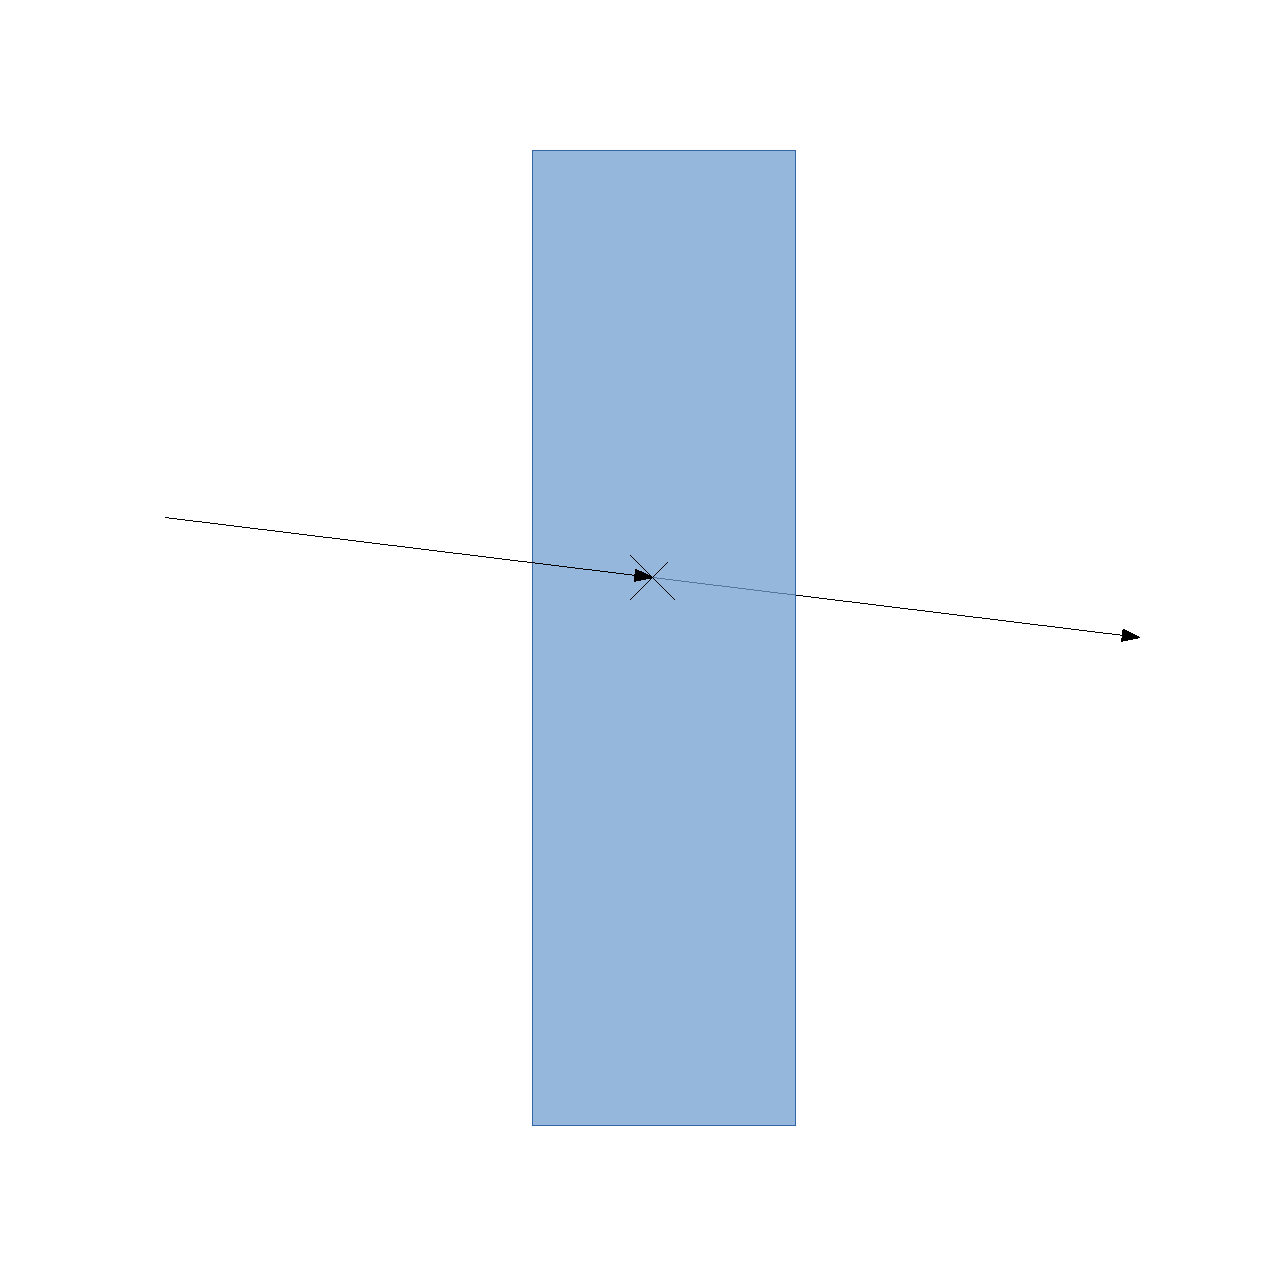
\includegraphics[angle=0,width=4in]{figures/bz.pdf}
      \caption{Graphical example of a decision tree.}
      \label{fig:dtree}
    \end{figure}
    
    A single tree can easily overfit a data set if it is at all complex, and
    its output is just a class label. Gradient-boosting addresses both of these
    issues by combining many weak classifiers into a strong one. Each weak
    classifier is built based on the error of the previous one. For a given
    training set, whenever a sample is classified incorrectly by a tree, that
    sample is given a higher importance when the next tree is being created.
    Mathematically, each tree is training on the gradient of the loss function.
    After all of the trees have been created, each tree is given a weight based
    on its ability to classify the training set, and the output of the
    gradient-boosted decision tree classifier is the probability that a sample
    is in a given class.
    
    The gradient-boosted decision tree software package we use is
    XGBoost~\cite{xgboost}. There are two types of classifiers we can use to
    separate protons from other tracks: binary and multiclass. Both classifiers
    are trained on all types of reconstructed tracks. A binary classifier
    classifies each track as either a proton or not a proton, and a multiclass
    classifier classifies a track as one of many types including a proton. We
    choose to use multiclass because the information about non-proton tracks is
    useful for event identification. The five classes that we train the
    decision trees to classify are protons (both BNB and cosmic), BNB muons,
    BNB pions, BNB electrons/photons, and all non-proton cosmics.
    
    The decision trees were trained to select protons in general. The target
    class contains all protons from BNB interactions, as well as cosmic
    protons. However, the choice of track features and most of the improvements
    that were made were done with the goal of a high efficiency for isolated
    protons and cosmic rejection.

  \subsubsection{Training}
    Describe the training sets. What samples were used, how many of everything,
    and all hyperparamter settings. Describe hyperparameter optimization. 
  \subsubsection{Performance}
    Show efficiency, accuracy, itemize backgrounds.
    Discuss reasons for different backgrounds.
  \subsubsection{Event selection}
    Need to select both NCE and CCQE events.
    Use particle ID plus reconstructed flashes.
    Exactly how we select NCE events 

%%%%%%%%%%%%%%%%%%%%%%%%%%%%%%%%%%%%%%%%%%%%%%%%%%%%%%%%%%%
% Efficiency and Background Estimation
%%%%%%%%%%%%%%%%%%%%%%%%%%%%%%%%%%%%%%%%%%%%%%%%%%%%%%%%%%%
\subsection{Efficiency and Background Estimation}\label{background}
  \subsubsection{Event selection efficiency}
    Efficiency due to TPC, PMT software trigger, reconstruction, proton ID,
    event selection, etc. This includes efficiency due to proton reinteracting
    in the nucleus and other nuclear effects.
  \subsubsection{Beam Induced Dirt Background}
    Discuss dirt neutrons, how they happen and estimated rates and energy
    distributions.  Show how well we can seperate or understand them. Show any
    sort of data-driven correction we did to dirt neutron background and how it
    affects our uncertainty. Talk about how well we can tag cryostat neutrons
    with the PMTs.
  \subsubsection{Beam Induced TPC Background}
    Talk about neutral-current elastic neutrons that are produced in the TPC
    and how their distributions differ from NCEp ones. Also include BNB
    backgounds (CCQE where muon wasn't reconstructed, NCpi0, etc.) Discuss how
    the optical signal would be different for each of these.
  \subsubsection{Cosmic Background}
    Discuss the difference between cosmic tracks and beam proton tracks. How do
    we separate them? What is the rate?

%%%%%%%%%%%%%%%%%%%%%%%%%%%%%%%%%%%%%%%%%%%%%%%%%%%%%%%%%%%
% Ratio of Cross Sections
%%%%%%%%%%%%%%%%%%%%%%%%%%%%%%%%%%%%%%%%%%%%%%%%%%%%%%%%%%%
\subsection{Ratio of NCEp to CCQEn Cross Sections}\label{ratios}
  Show how the ratio gets rid of a lot of measurement uncertainty like beam
  flux and efficiencies. Give exact equation that we will be using for
  analysis. Show how $\Delta s$ is still large at low $Q^2$.
  \subsubsection{Sources of Measurement Uncertainty}
    TPC efficiency: If ionization electrons actually reach the
    TPC and leave a signal.
    PMT trigger efficiency: Refer back to PMT trigger studies. Give uncertainty
    due to on signal.
    Reconstruction efficiency: Refer back. Give uncertainty on signal.
  \subsubsection{Quantifying Uncertainty on Ratio}\label{errorcalc}
    Calculate exact uncertainty and show it here.
  \subsubsection{}
    Nuclear effects and FSI. Discuss 

%%%%%%%%%%%%%%%%%%%%%%%%%%%%%%%%%%%%%%%%%%%%%%%%%%%%%%%%%%%
% Comparison to Simulation
%%%%%%%%%%%%%%%%%%%%%%%%%%%%%%%%%%%%%%%%%%%%%%%%%%%%%%%%%%%
\subsection{Comparison of data to simulation}
  \subsubsection{Reweighting}
  \subsubsection{Likelihood calculation}

%%%%%%%%%%%%%%%%%%%%%%%%%%%%%%%%%%%%%%%%%%%%%%%%%%%%%%%%%%%
% Joint Estimation
%%%%%%%%%%%%%%%%%%%%%%%%%%%%%%%%%%%%%%%%%%%%%%%%%%%%%%%%%%%
\subsection{Strange axial form factor parameter estimation}\label{deltas}
  Here is where we do the actual MCMC.
  \subsubsection{Bayesian inference}
    Walk through the Bayesian math. Start with wanting the probability of
    $\theta$ given the data and the model and get final equation. Then show how
    to combine with previous experiments. Should give detail for each factor in
    equation (prior, likelihood, posterior, evidence). Should especially give
    detail on how we choose priors. Maybe talk about model selection when
    talking about the evidence.
  \subsubsection{Markov Chain Monte Carlo}
    Go through detail on our implementation of MCMC. Discuss how Markov Chains
    work in general. Describe Metropolis, Gibbs, and our combination of both.
  \subsubsection{Results}
    Lots of plots! $\Delta s$!


%This is the end of analysis section

\newpage
%\section{SAMPLE TEXT WITH GRAPHICS} \label{graphics}
%This file illustrates how include in your thesis graphical
 %output.
%The next line produces an indented paragraph to start the document
 %unit.  The LaTeX defaults start most units without indentations.
\hspace{\parindent}
This is sample text with graphics.
\begin{figure}[h]
  \centering
  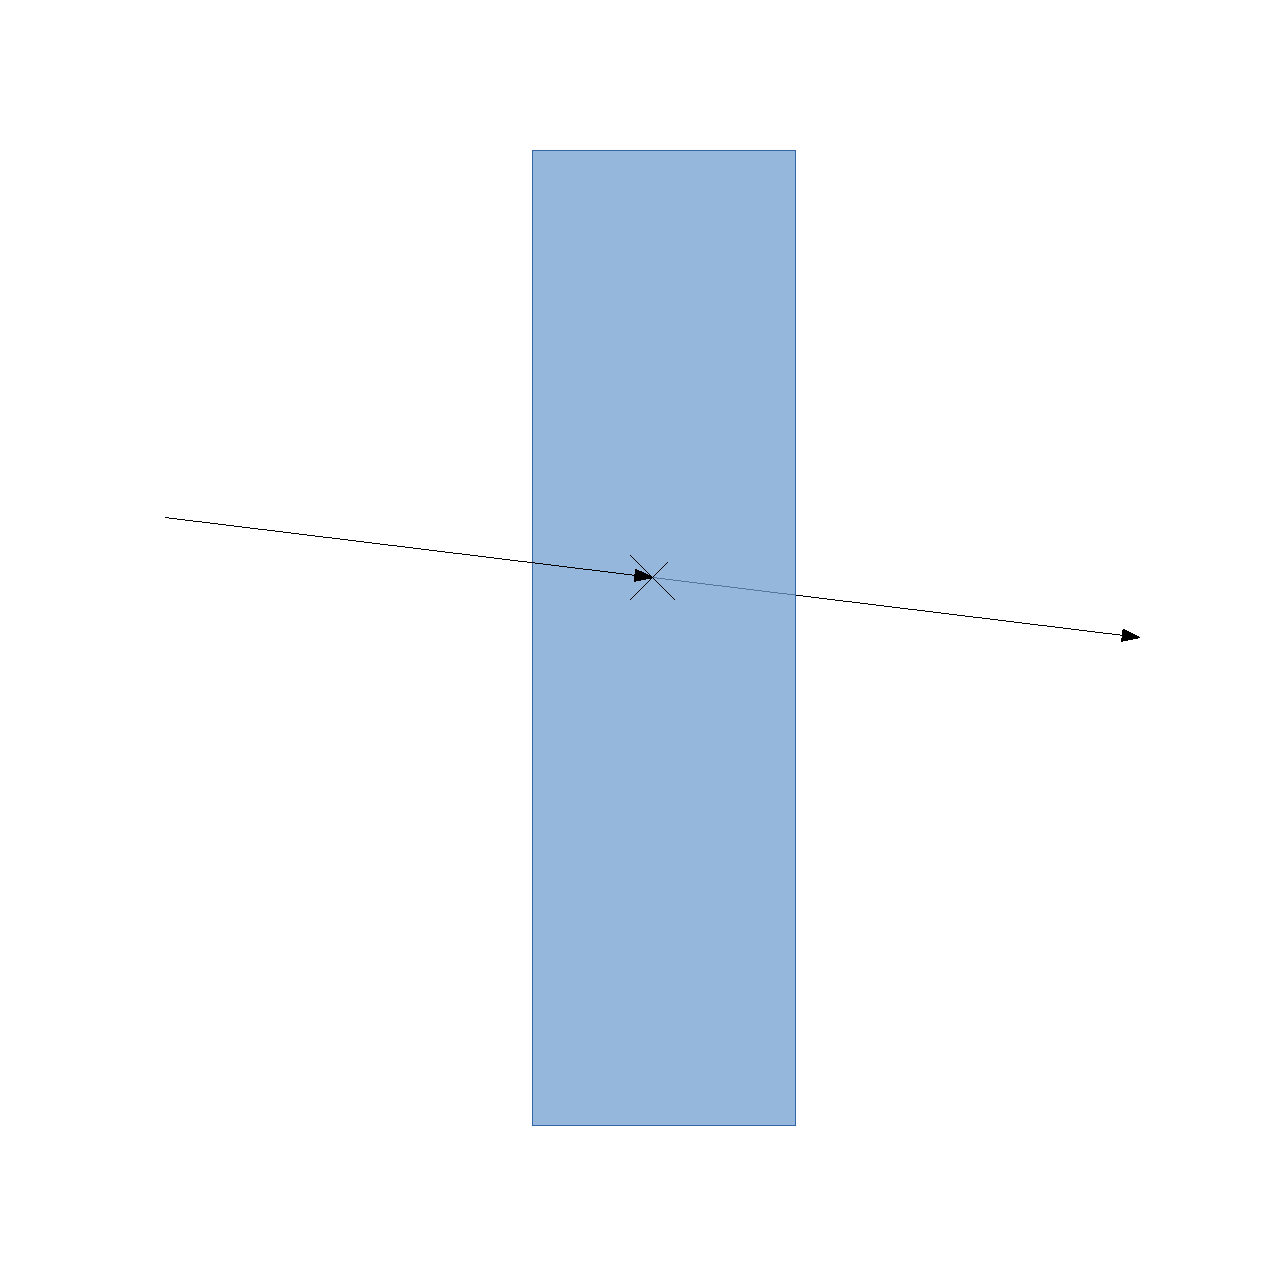
\includegraphics[angle=-90,width=4in]{figures/bz.pdf}
  \caption{This is an inserted EPS graphic}
  \label{fig:mygraph1}
\end{figure}
Sample ref of \ref{fig:mygraph1} 

\begin{figure}[t]
 \centering
  \includegraphics[angle=-90, width=4in]{figures/E734eta.pdf}  
    \caption{This is another inserted PDF graphic}
    \label{fig:mygraph2}
\end{figure}
%This is the end of the file graphics.tex


%\newpage
%The next four lines create a list of references for the 
 %paper from a .bbl file created by BibTeX from a .bib bibliographic
 %database file.  
 %The MathSciNet clipboard was used to prepare 
 %the .bib file.  See Lamport's book mentioned in the references for
 %basic information about BibTeX.  If you don't use BibTeX, you need
 %to create and format the list of references yourself.
\addcontentsline{toc}{section}{REFERENCES}
\setlength{\baselineskip}{\singlespace}
\bibliographystyle{plain}
\bibliography{main}
%These next three command lines create a list of references for the paper from
 %a biblio.tex file you create yourself.
%\addcontentsline{toc}{section}{REFERENCES}
%\setlength{\baselineskip}{\singlespace}
%%This file is a list of references prepared by hand.  If you are going 
 %to prepare your list of references by hand, you need to look
 %carefully at a journal and try  %to follow consistently the
 %journal's style.  
\begin{thebibliography}{99}

\bibitem{loday2} Fiedorowicz, Zbigniew  and Loday, Jean-Louis.
{\em Crossed Simplicial Groups and Their Associated Homology.}
Transactions of the American Mathematical Society, {\bf 36}(1991), p 57-87.

\bibitem{Higham}
Higham, Nicholas, J.  
{\em Handbook of writing for the mathematical sciences}, second edition.
Society for Industrial and Applied Mathematics, 1998.

\bibitem{Lamport} Lamport, Leslie.
{\em LaTeX:  A Document Preparation System}, Second Edition.
Addison-Wesley, (1994).

\bibitem{Lodaybook}Loday, Jean-Louis.
{\em Cyclic Homology.}
Springer Verlag, (1992).

\bibitem{L-Q} Loday, Jean-Louis and Quillen, Daniel.
{\em Cyclic Homology and the Lie Algebra Homology of Matrices.}
Comment. Math. Helv. {\bf 59}(1984), p 565-591.

\bibitem{Reckdahl}  Reckdahl, Keith.
{\em Using EPS Graphics in \LaTeX\ $2_{\varepsilon}$ Documents}.
Preprint, 1997.
 
\bibitem{Swanson}  Swanson, Ellen.
{\em Mathematics into type,} revised edition.
American Mathematical Society, 1979.

\end{thebibliography}
%This is the end of the file biblio.tex














%
\end{document}
